\section{Kiste auf schiefer Ebene}
\begin{figure}
  \centering
  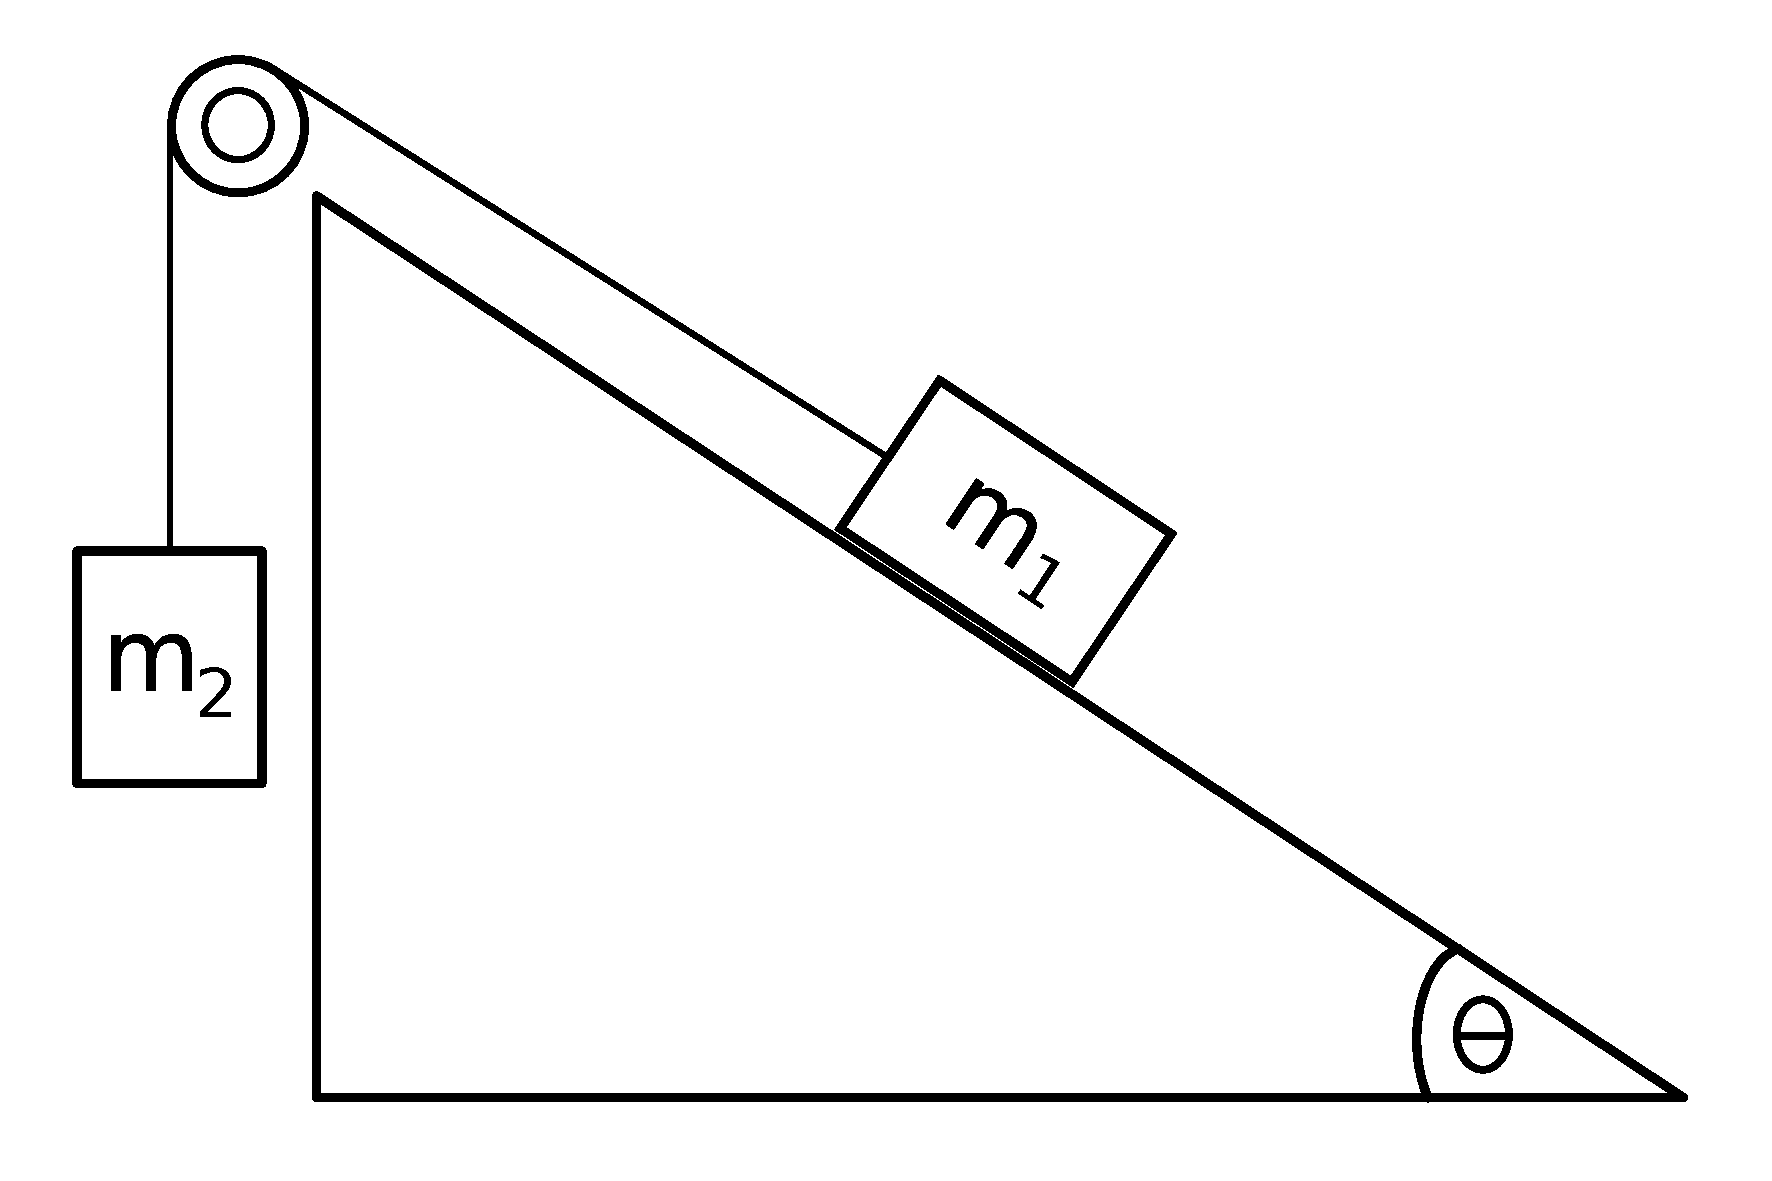
\includegraphics[width=0.65\textwidth]{aufg1.pdf}
  \label{fig: aufg1}
\end{figure}


Eine Kiste der Masse $m_1 = 10 \si{\kilo\gram}$ befindet sich auf einer schiefen Ebene mit dem Winkel $\Theta = 36.9\si{\degree}$.
Sie ist über eine Umlenkrolle mit einem Gegengewicht der Masse $m_2$ verbunden. Der Haftreibungskoeffizient sei $\mu_H = 0.4$ und
der Gleitreibungskoeffizient sei $\mu_G = 0.3$.
  \begin{enumerate}[label=\roman*]
    \item Für welche Werte der Masse $m_2$ ist das System in Ruhe?
    \item Nun sei $m_2 = 10\si{\kilo\gram}$. Wie stark werden die beiden Kisten beschleunigt?
  \end{enumerate}
Verwende: $\sin\left(36.9\si{\degree}\right) = 0.6,\, \cos\left(36.9\si{\degree}\right) = 0.8$, sowie $g = 9.8 \si{\meter \per \second^2}$

\newpage
